\clearpage

\section{SystemArkitektur}

\subsection{SysML} 

\begin{figure}[h]
	\centering \resizebox{\textwidth}{!}{
	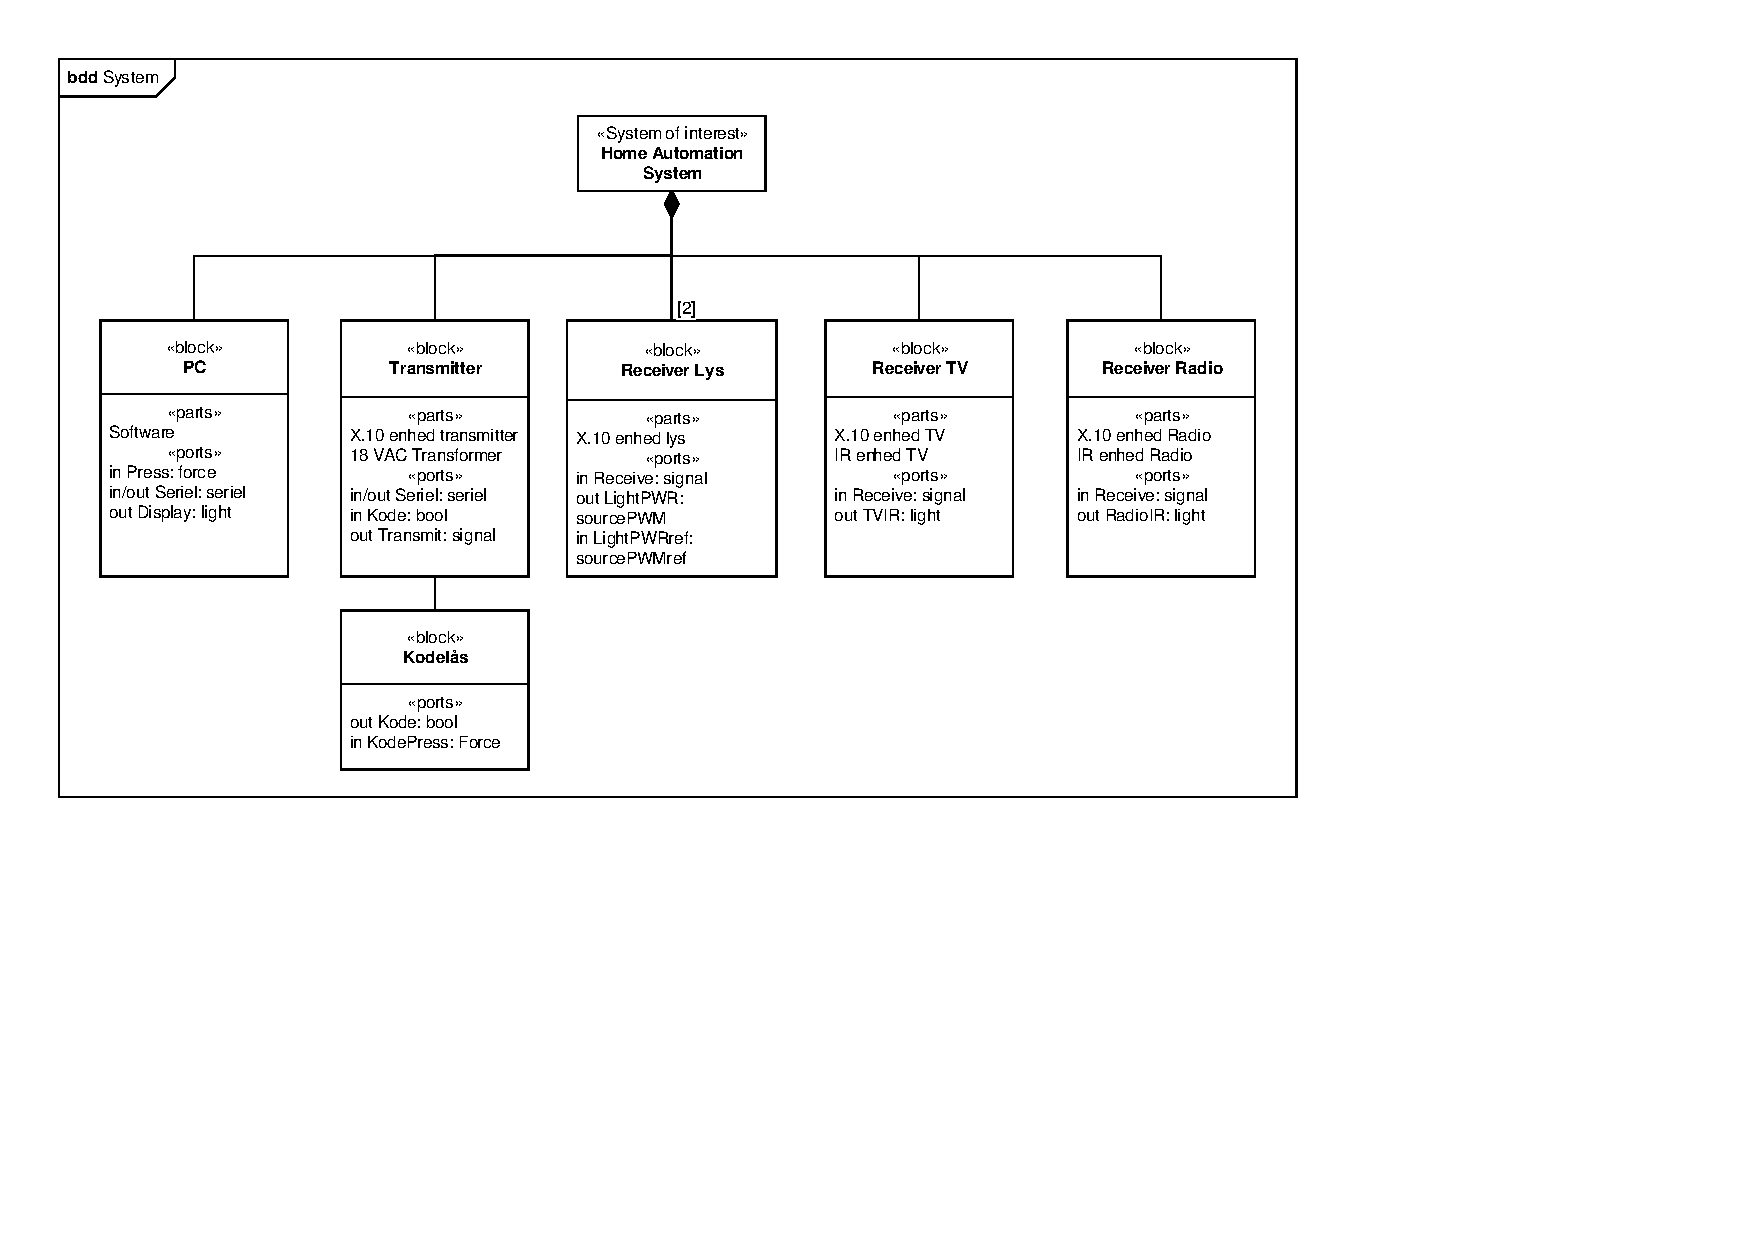
\includegraphics[scale=1,trim=28 210 219 25, clip=true]{Projektbeskrivelse/Systemarkitektur/diagrammer/BDD_System.pdf}}
	\caption{BDD diagram for systemet}
\end{figure}

I systemarkitekturen blev der lavet blokke for alle elementer, og det blev forklaret hvad disse enkelte blokke består af. Dette hjalp til at give et bedre overblik over systemet. BDD'er og IBD'er er anvendt fra ISE undervisningen. BDD'erne er brugt til at beskrive, hvilke komponenter systemet består af, og som det ses på overståene BDD-diagram, er der lavet en blok for hver del: PC, Transmitter, Receiver lys, Receiver tv og Receiver radio.

IBD'erne er brugt til at vise signaltyper mellem blokkene, derudover beskriver de også systemets forbindelser. Forbindelserne har i hver sin ende nogle flowports, disse bruges til at synliggøre signalets retning og sammenhæng med andre flowporte. For hvert enkelt blok er udarbejdet en IBD, så det under design fasen er nemt at se sammenkoblingen mellem de enkelte elementer.

På baggrund af IBD'erne blev der udarbejdet en signalbeskrivelse, som ved hjælp af diverse datablade sikrer at systemet overholder alle elementernes tolerancer, så der ikke bliver ødelagt noget.

\subsection{Applikationsmodel}

Applikationsmodellen var valgt primært for softwareudviklernes skyld, da det gav en systematisk måde at opbygge softwareklasser på. Ved at se Use Cases igennem, blev der fundet konceptuelle klasser, som igen blev brugt til at bestemme hvilke kllasser, der gav mening at oprette. Efter klasserne var valgt, blev de klassificeret yderligere i hhv. boundary-, domain- og controllerklasser. Disse bruges til at holde styr på, i hvilke klasser funktionaliteten skal være.
Herefter blev der lavet sekvensdiagrammer, hvori der tages udgangspunkt i en Use Case, så metoder kan findes ud fra, hvad der skal ske for at den pågældende Use Case bliver opfyldt.

\clearpage